\documentclass[11pt,a4paper]{article}

\usepackage[parfill]{parskip}
\usepackage{subfig}
\usepackage{amsmath}
\usepackage{makeidx}
\usepackage{graphicx}
\usepackage[bibstyle=numeric, citestyle=numeric-comp]{biblatex}
\usepackage{multicol}
\usepackage{letltxmacro}
\usepackage{listings}
\DeclareGraphicsExtensions{.pdf,.png,.jpg}

%\addbibresource[location=remote]{C:/Users/CptProton/Documents/Bibliographies/Labs.bib}

\LetLtxMacro{\oldsqrt}{\sqrt} % makes all sqrts closed
\renewcommand{\sqrt}[1][]{%
  \def\DHLindex{#1}\mathpalette\DHLhksqrt}
  \def\DHLhksqrt#1#2{%
    \setbox0=\hbox{$#1\oldsqrt[\DHLindex]{#2\,}$}\dimen0=\ht0
    \advance\dimen0-0.2\ht0
    \setbox2=\hbox{\vrule height\ht0 depth -\dimen0}%
    {\box0\lower0.71pt\box2}}

    \makeatletter
    \newenvironment{tablehere}
    {\def\@captype{table}}
    {}

    \newenvironment{figurehere}
    {\def\@captype{figure}}
    {}
    \makeatother

    \title{Automatic Fingerprint Recognition}
    \author{Benjamin May \& Edward Wastell}
%\date{}

    \begin{document}
    \maketitle

    \begin{abstract}
      Stuff happened.
    \end{abstract}

    \begin{multicols}{2}

\section{Introduction}
	Fingerprints have been used to identify people since the 19\textsuperscript{th} century and have been used in criminal investigations since about that time. More recently fingerprints have been used as biometric markers used in boarder control, library stock control and computer and building access control systems. The need for a robust automatic fingerprint recognition system is obvious.

	Most fingerprint recognition systems in use are based on the idea of identifying minutiae (points where a ridge ends or joins with another ridge) --- in this article a system that uses the greylevel gradient to find minutiae is discussed.

        Traditionally, fingerprint analysis consisted of first processing the image in some way, usually either binarization or line thinning. Methods like this have two major drawbacks. Firstly, such alterations to the image can be computationally expensive and therefore take a considerable amount of time for large images, which is a serious problem when used in real time applications. Secondly, non-reversible image manipulation can lead to destruction of information about the fingerprint.


\section{Theory and Implementation}


        The method used in the article does not rely on prior image manipulation. It works by think of the image as a three dimensional object, with the greylevel of time image being the height in the Z-direction. The tangent of this object is then calculated at the position of each pixel in the image. A line can then be traced along the image by taking steps in the direction orthogonal to these tangents. By building up such lines from different starting points in the image, we can classify the entirety of the fingerprint. The two types of minutia we are looking for can be found from this complete classification. Where a line ends without touching another line or the edge of the image is a termination and points where one line hits the middle of another are bifurcations.


	\subsection{Point Normal Direction}
\begin{figure*}
\centering
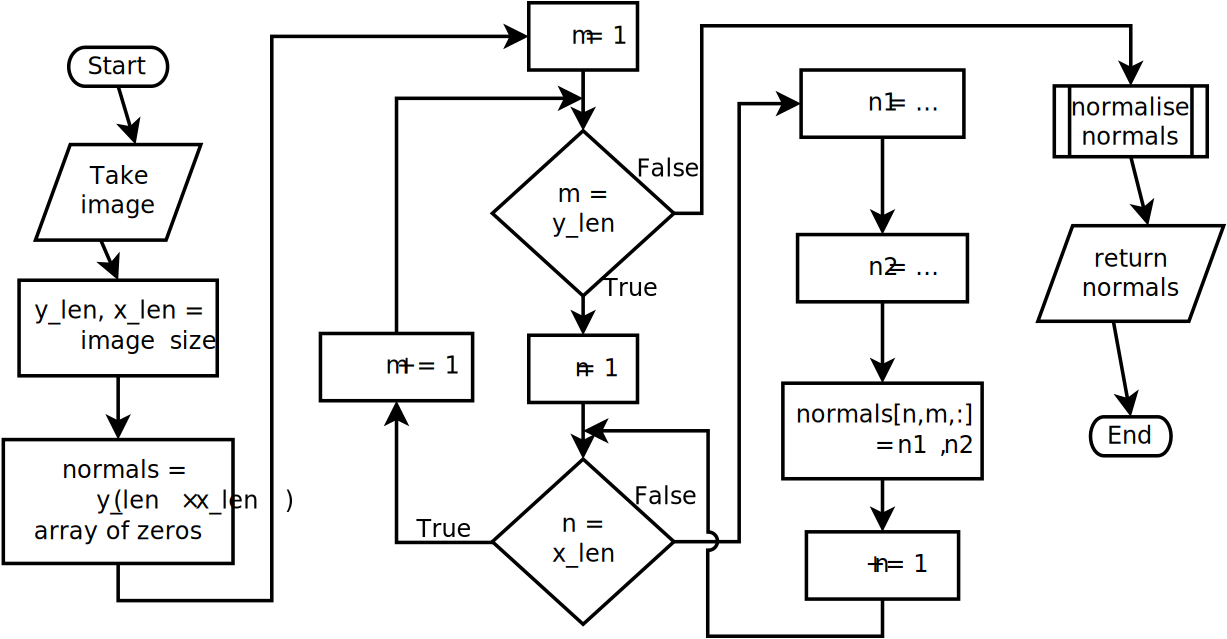
\includegraphics[width = \textwidth]{PND}
\caption{Flow chart of the PND function as implemented.}
\label{fig:PND-alg}
\end{figure*}


		The point normal function works by taking four mutually adjacent points (\textit{i.e.} a $2 \times 2$ array of pixels) and fitting a plane to them. If the greylevel at the pixel $(x_k, y_k)$ is denoted $h_k$ and the level from the fitted plane is denoted $p_k$ then the plane fitting part of the function can be seen as minimising the following expression:

		\begin{equation}
			\min_{n_1, n_2, c} \sum_k |h_k - p_k|^2
		\end{equation}
		
		Which in matrix form can be expresed as:

		\begin{equation}
			\begin{vmatrix}
			\begin{pmatrix}
			h_1 \\
			h_2 \\
			h_3 \\
			h_4
			\end{pmatrix}
			-
			\begin{pmatrix}
			-x_1 & -y_1 & 1 \\
			-x_2 & -y_2 & 1 \\
			-x_3 & -y_3 & 1 \\
			-x_4 & -y_4 & 1
			\end{pmatrix}
			\begin{pmatrix}
			n_1 \\
			n_2 \\
			c
			\end{pmatrix}
			\end{vmatrix}^2
		\end{equation}

		Where $n_1$, $n_2$ and $c$ are the $x$, $y$ and $z$ components of the surface normal respectively. This is a simple least-squares minimisation and after some rearranging we obtain the following expressions for the optimum surface normal:

		\begin{equation}
		\begin{split}
			n_1 = \frac{-h_1 + h_2 + h_3 - h_4}{4} \\
			n_2 = \frac{-h_1 - h_2 + h_3 + h_4}{4} \\
			c = \frac{h_1 + h_2 + h_3 + h_4}{4}
		\end{split}
		\end{equation}

		Since we are only concerned with the components in the $x,y$--plane the function implemented here doesn't bother calculating $c$ (figure \ref{fig:PND-alg}). Once all $2 \times 2$ neighbourhoods have been fitted the function returns $n_1$ and $n_2$ then terminates.

		As the NPD function needs a four points to fit a plane to the decision has to be made regarding how edges are handled. One possibility is to `wrap' the edges of the image around, effectively forming a torus --- this was not implemented here because it would mean that for two edges the values of $n_1$ and $n_2$ would depend on greylevels from the other two edges. The second possibility (implemented here) is to make the output array smaller by 1 pixel in both dimensions, so if the original image is $n \times m$ pixels the array of normals is $(n-1) \times (m-1)$. From figure \ref{fig:PND-alg} it can be seen that the PND function implemented here loses the top and right hand pixels.

	\subsection{Averaged Tangent Direction}
        \begin{figure*}
        \centering
        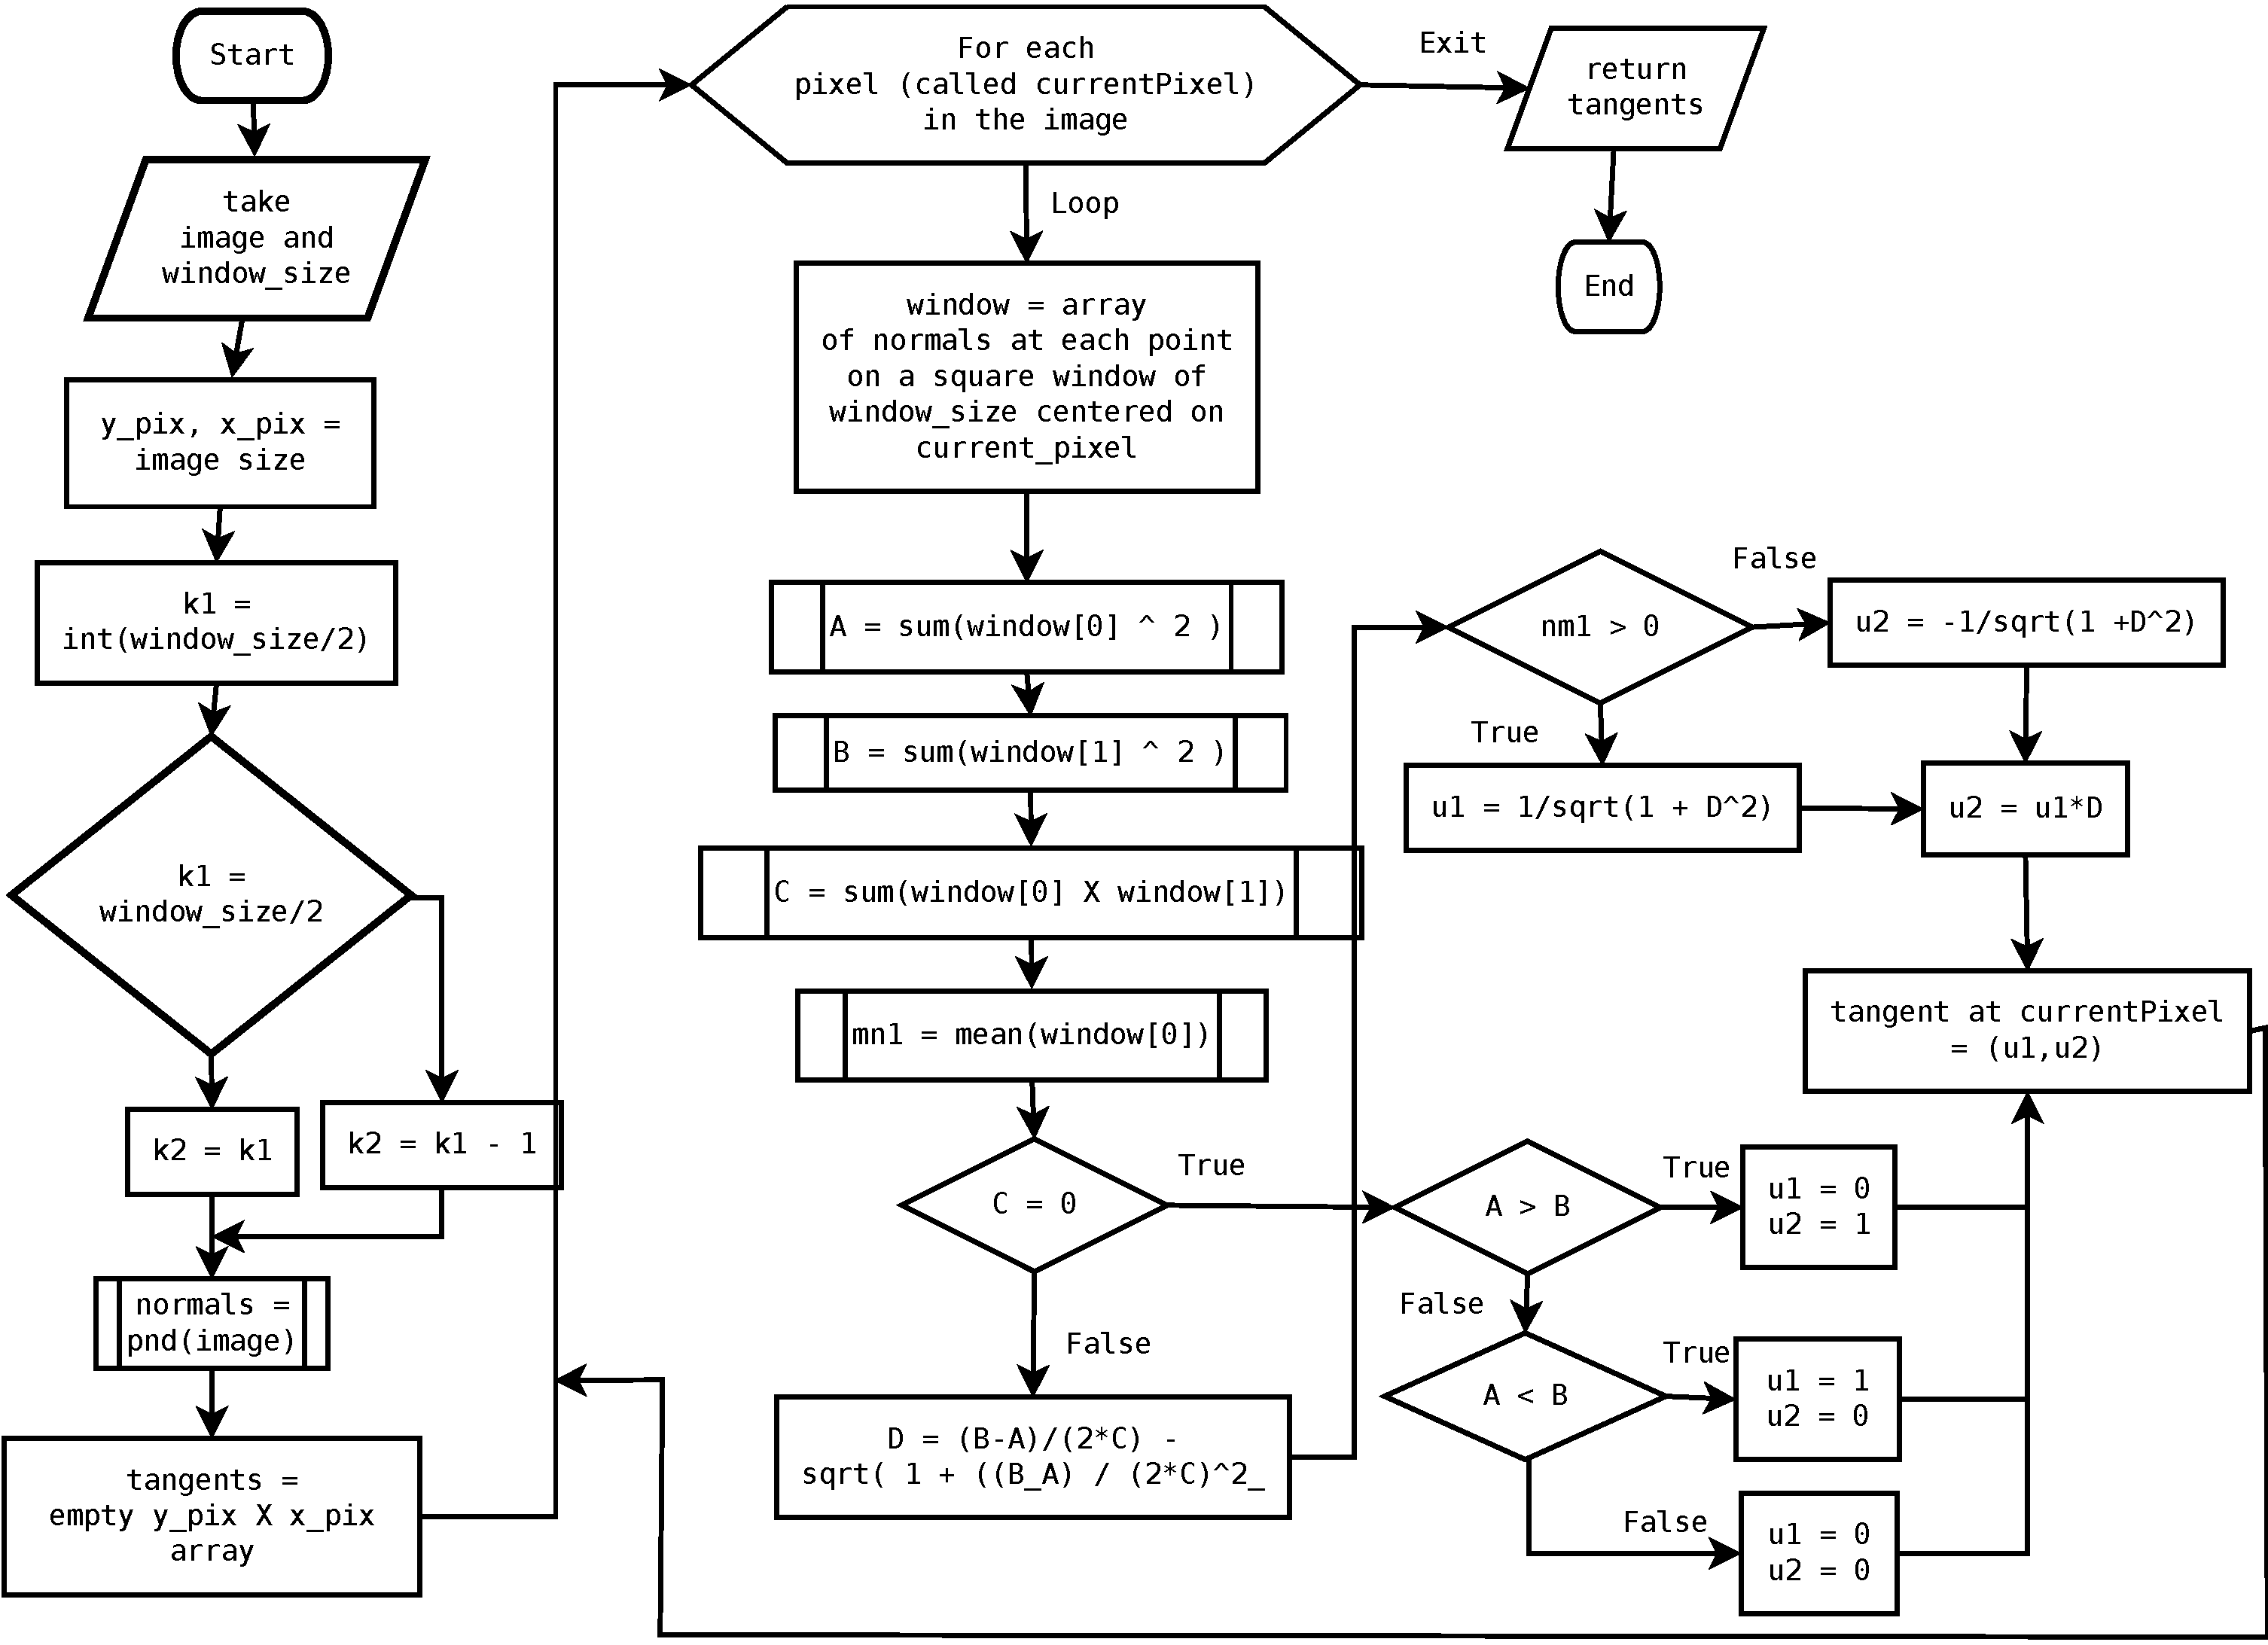
\includegraphics[width = \textwidth]{ATD.pdf}
        \caption{Flow chart of the ATD function as implemented.}
        \label{fig:ATD-alg}
      \end{figure*}
		The ATD function calculates the $x,y$--plane tangent that best fits with the surface normals generated by the PND function in a given $n \times n$ neighbourhood. This has the effect of smoothing out (plane normal angle) noise but, as with analogous smoothing operations, can obscure features with a size comparable to that of the kernel chosen. The fitting is a least squares minimisation of the row-by-row dot product:

		\begin{equation}
		\begin{split}
			\min_{u_1, u_2} \sum_k |(n_{1,k}, n_{2,k}) \cdot (u_1, u_2)|^2 \\
			= U(u_1, u_2)
		\end{split}
		\end{equation}

		Where $n_{1,k}$ is the $k$\textsuperscript{th} $n_1$ value as defined above \textit{e.t.c.} and $(u_1, u_2)$ is the normalised fitted vector. If we define the following:

		\begin{equation}
		\begin{split}
			A = \sum_k (n_{1,k})^2 \\
			B = \sum_k (n_{2,k})^2 \\
			C = \sum_k n_{1,k} n_{2,k}
		\end{split}
		\end{equation}

		then we can express $U(u_1, u_2)$ as

		\begin{equation}\label{eq:U_mat}
		\begin{split}
			U(u_1, u_2) = \\ (u_1, u_2)
			\begin{pmatrix}
			A & C \\
			C & B
			\end{pmatrix}
			\begin{pmatrix}
			u_1\\
			u_2
			\end{pmatrix}
		\end{split}
		\end{equation}

		The eigenvalues of the above $2 \times 2$ matrix, $\lambda_1$ and $\lambda_2$, are the maximum and minimum values of $U$ respectively. It is trivial to determine that the two eigenvalues are given by:

		\begin{equation}
		\begin{split}
			\lambda_1 = \frac{A + B + \sqrt{(A - B)^2 + 4C^2}}{4} \\
			\lambda_2 = \frac{A + B - \sqrt{(A - B)^2 + 4C^2}}{4}
		\end{split}
		\end{equation}

		With some further rearranging of equation \eqref{eq:U_mat} we find that:

		\begin{equation}\label{eq:ATD_u}
			u_1 = \sqrt{\frac{1}{1 + \left(\frac{\lambda_2 - A}{C}\right)^2}}
		\end{equation}

		\begin{equation}
			u_2 = u_1 \left(\frac{\lambda_2 - A}{C}\right)
		\end{equation}

		In implementing these equations several special cases have to be taken into account. The first special case is when $C = 0$, which would require deviding by zero. To cope with this case the function is set to test if $C = 0$ and if so the function will set $(u_1, u_2) = (1,0)$ or $(u_1, u_2) = (0,1)$ depending on weather $A < B$ or $B > A$ respectively. The second special case is  when $\lambda_1 = \lambda_2$, which the function tests for after determining if $C = 0$. In this case there is no optimum orientations thus $(u_1, u_2) = (0,0)$.

		A final problem with implementing equation \eqref{eq:ATD_u} is the fact that $u_1$ can only ever be positive. This ensures that in the $x$--direction one cannot distinguish between the two sides edges of a ridge. To solve this the function calculates the mean of the $n_1$ values then checks if this mean is negative and if so it makes $u_1$ negative.

	\subsection{The Ridge Follower}
		The ridge following system takes a slice (of width $2 \sigma + 1$ and height 1 pixel centred around pixel $(x_c, y_c)$) of the image, finds the peak of the ridge and moves to it, calculates the direction of the ridge ($\phi_c$) then moves forward by $\mu$ pixels before starting the process again (figure \ref{fig:ridge_follow_simpled}). In this manor the ridge follower follows the ridge, and since the function logs where it's been it's possible to determine where the minutiae are.

\begin{figurehere}
\centering
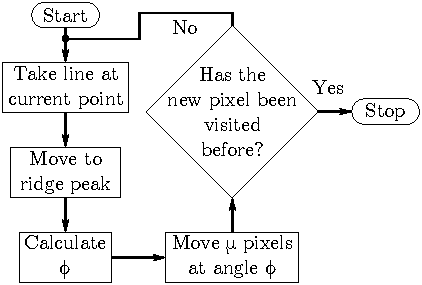
\includegraphics[width = 0.48\textwidth]{ridge_follow_simpled}
\caption{Simple version of the ridge following algorithm.}
\label{fig:ridge_follow_simpled}
\end{figurehere}

		Taking a line at a given point is simple enough: the current pixel, $(x_c, y_c)$, is the centre of the line and by simple trig the coordinates of the pixels that make up the line are

		\begin{equation}
		\begin{split}
			\begin{pmatrix}
			x_{l,k} \\
			y_{l,k}
			\end{pmatrix}
			= \\
			\begin{pmatrix}
			x_c \\
			y_c
			\end{pmatrix}
			+ (k - \sigma)
			\begin{pmatrix}
			\cos{(\phi_c + \pi/2)} \\
			\sin{(\phi_c + \pi/2)}
			\end{pmatrix}
		\end{split}
		\end{equation}

		where $x_{l,k}$ is $x$--coordinate of the $k$\textsuperscript{th} pixel of the line \textit{e.t.c.} and $k$ ranges from zero to $2 \sigma + 1$. Using these coordinates one can extract the relevant greylevels and plane normals.

		Identifying the peak of the ridge is somewhat involved if noise tolerance is needed. One method is to find the point midway between the two angles that are closest to the end of the lines. Another method is to try and smooth out the ridge to ensure that there is just one peak in it. 

In the algorithm employed here a more simplistic (and not as noise tolerant) method that simply finds the darkest point in the line.
			
\subsection{Minutia Detection}
        Once a complete set of ridges for the image has been found, the individual minutia can be defined. There are two types of minutia that we are interested in: terminations and bifurcations. Terminations occur where the end of a line is not at the edge of the image. This is fairly simple to detect: if a ridge ends and is more that $\mu$ pixels away from the edge of an image this will be a termination point. A bifurcation is when a single line splits into two lines. Attempting to find when a line splits can be difficult, as our ridge following algorithm will only follow one of two lines. However, it should be obvious that a line meeting the middle of another line is equivalent to a line branching. As the ridge following algorithm terminates if it finds an already visited pixel, it is possible to find positions where bifurcation may occur by looking at terminations. For each such point, we can extend the ridge follower by one more step. If this new point is already registered to another line, we can count this point as a bifurcation instead of a termination.

        If we know the location of all points of minutia and their type, we can in theory check whether two fingerprints are the same. Although it has not been proved that fingerprint minutia is sufficient to differentiate individuals, no two people have ever been found who have the same fingerprint minutia. There are a number of advantages to comparing a list of minutia as opposed to doing the same with a collection of images, the first of which is space. Although modern computers can store many high resolution images, a relatively small list of points is several orders of magnitudes smaller. The second reason is accuracy. It is unlikely that two pictures of fingerprints are exactly the same - there are many ways small errors in image acquisition can occur. If using exact picture matching, some on the fly processing must happen to get different images to be comparable, which can loose some information. Lastly, minutia matching should be faster. 
        \begin{figure*}
          \centering
          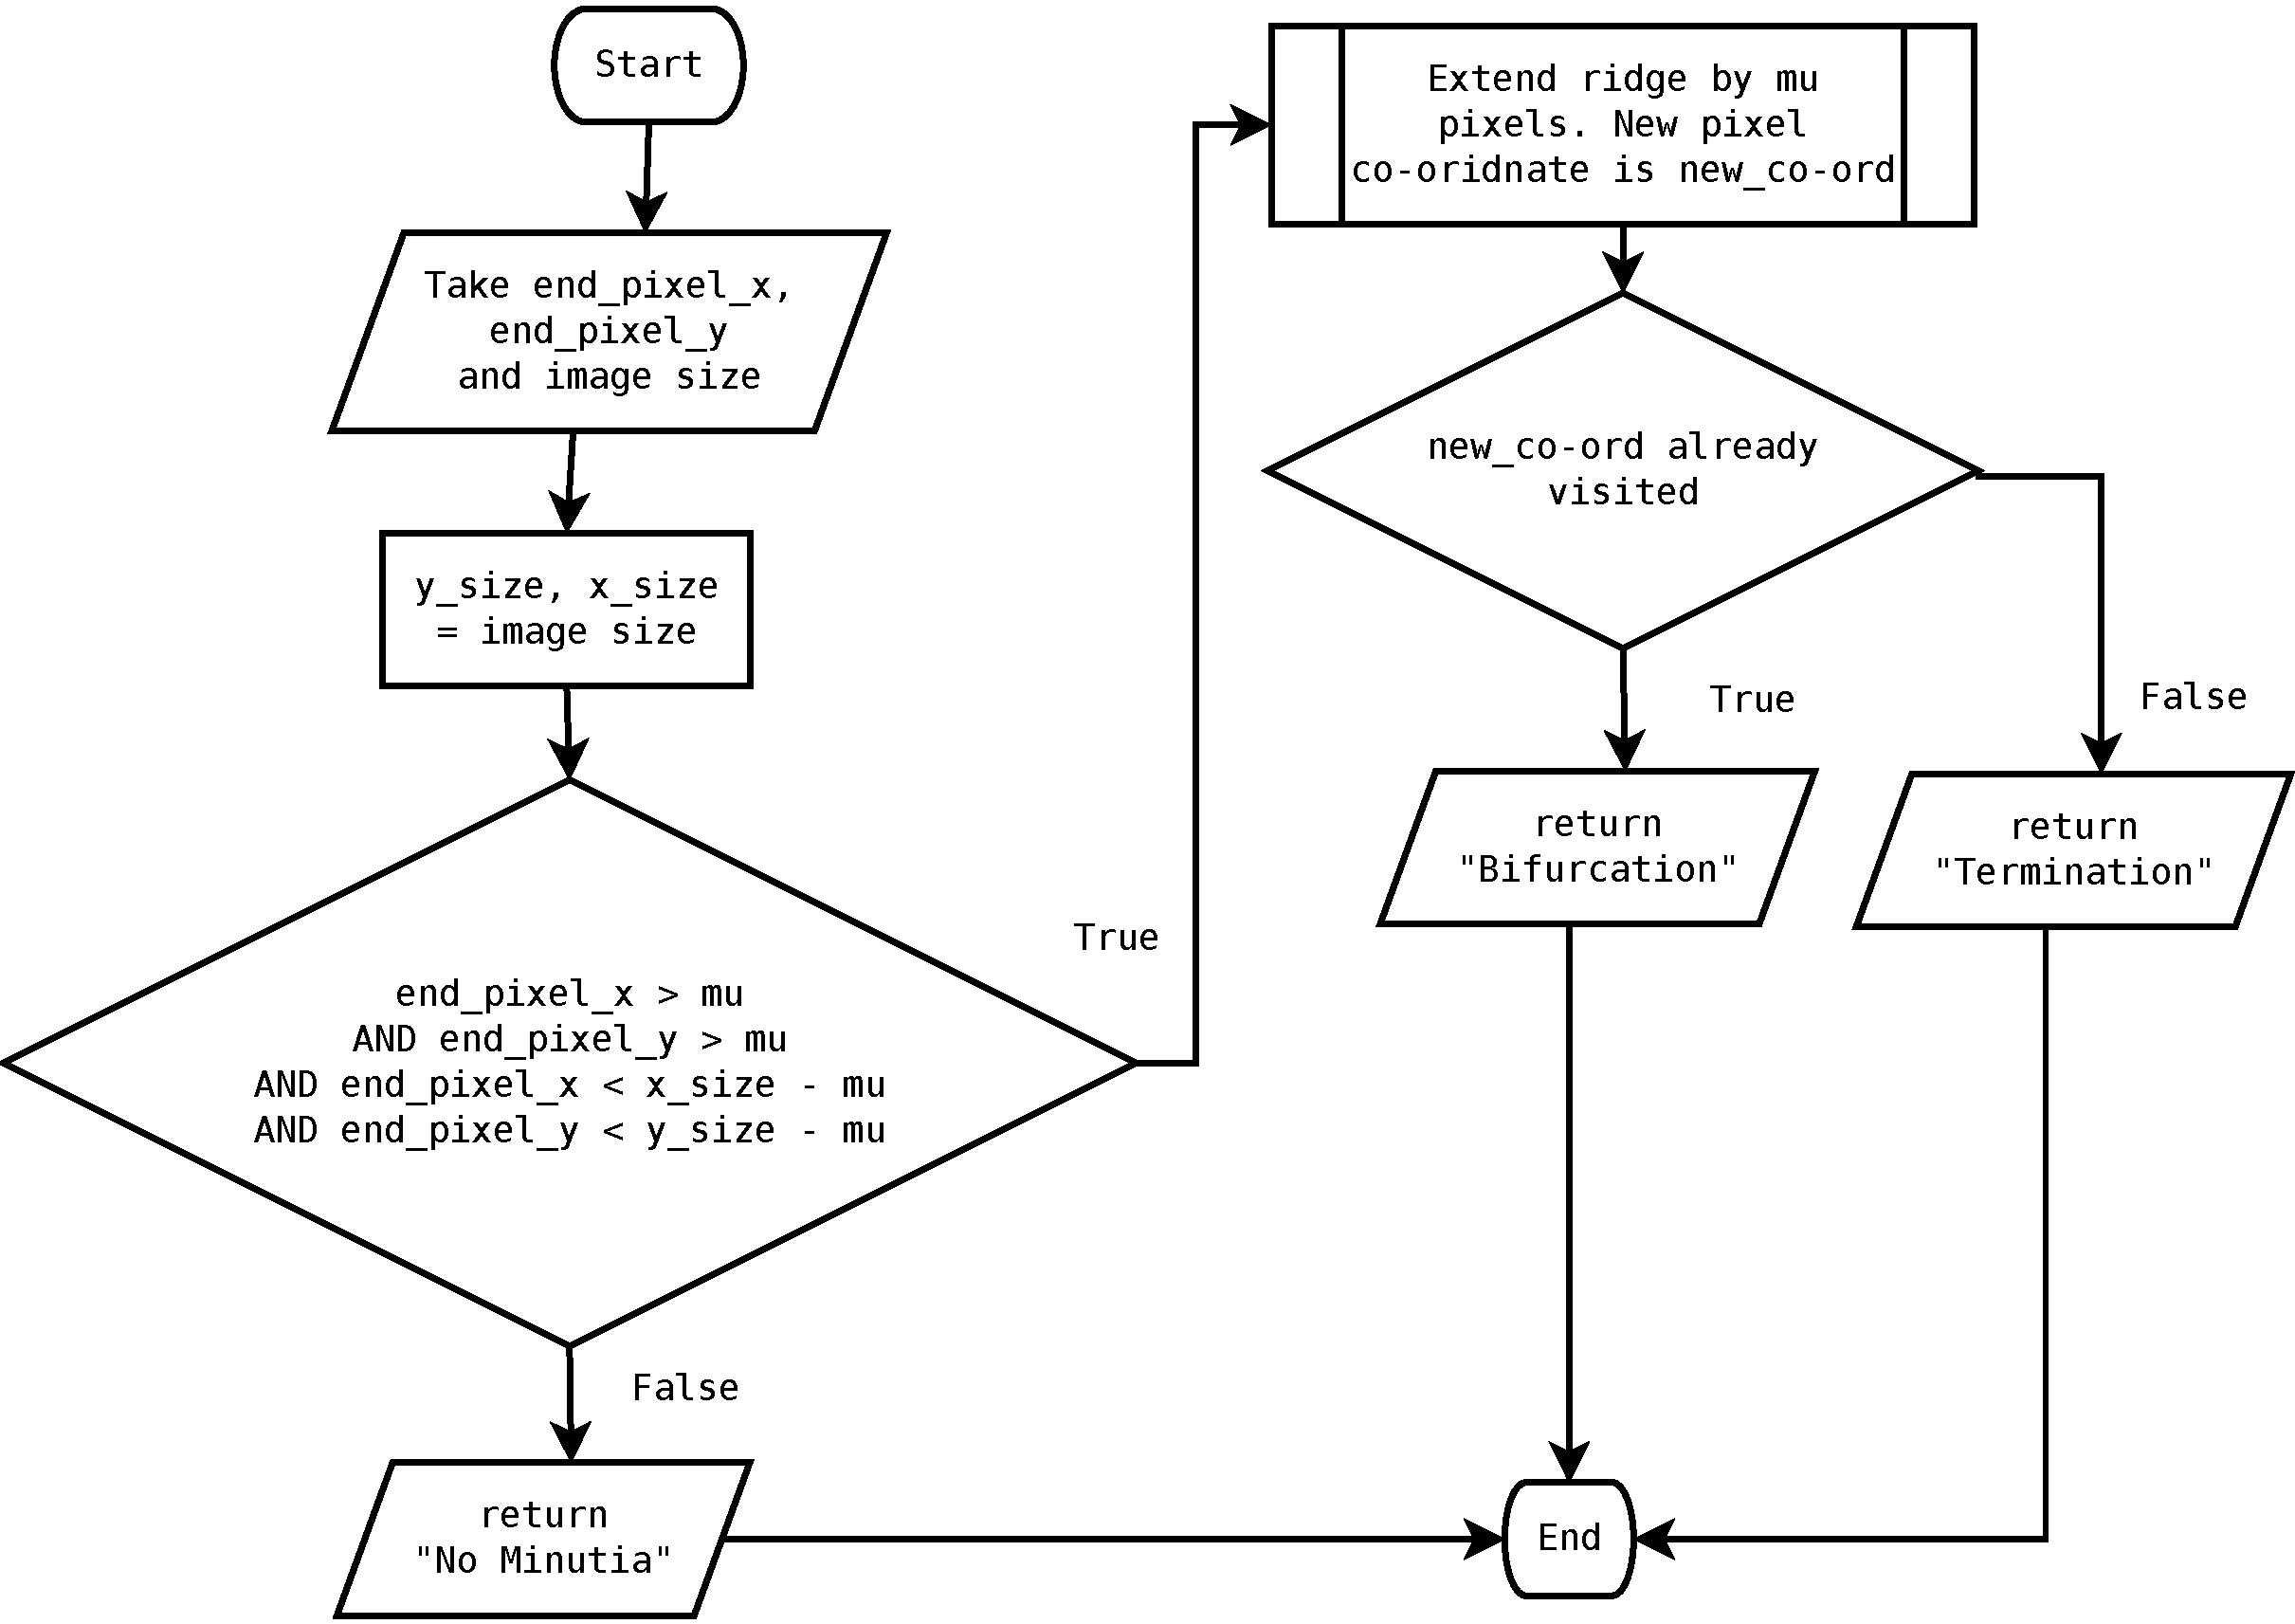
\includegraphics[width = \textwidth]{minutia.pdf}
          \caption{Flow chart for minutia detection. This is applied to the end of each ridge found.}
          \label{fig:min-alg}
        \end{figure*}

\section{Experimental Procedure}

\section{Results \& Analysis}

\section{Conclusion}


\printbibliography
\end{multicols}

\appendix
\section{Code}
	\lstinputlisting[language=Python]{../basic_code_elements.py}

\end{document}
